\documentclass{scrartcl}

\usepackage[utf8]{inputenc}


% zus�tzliche mathematische Symbole, AMS=American Mathematical Society 
\usepackage{amssymb}
\usepackage{amsmath}
\usepackage{amsthm}
\usepackage{bbm}
\usepackage{color}
\usepackage{listings}
\usepackage{pdfpages}
\usepackage{csquotes}

% f�rs Einbinden von Graphiken
\usepackage{graphicx}

% f�r Namen etc. in Kopf- oder Fu�zeile
\usepackage{fancyhdr}
\usepackage{tikz}
\usetikzlibrary{arrows, automata}

% erlaubt benutzerdefinierte Kopfzeilen 
\pagestyle{fancy}

% Definition der Kopfzeile
\lhead{
\begin{tabular}{lll}
Johannes Kalmbach &  &   \\
\end{tabular}
}
\chead{}
\rhead{\today{}}
\lfoot{}
\cfoot{Seite \thepage}
\rfoot{} 

\begin{document}

\section*{Deep Learning Lab, Report for Submission 2}

\subsection*{Exercise 2, Learning Rates}
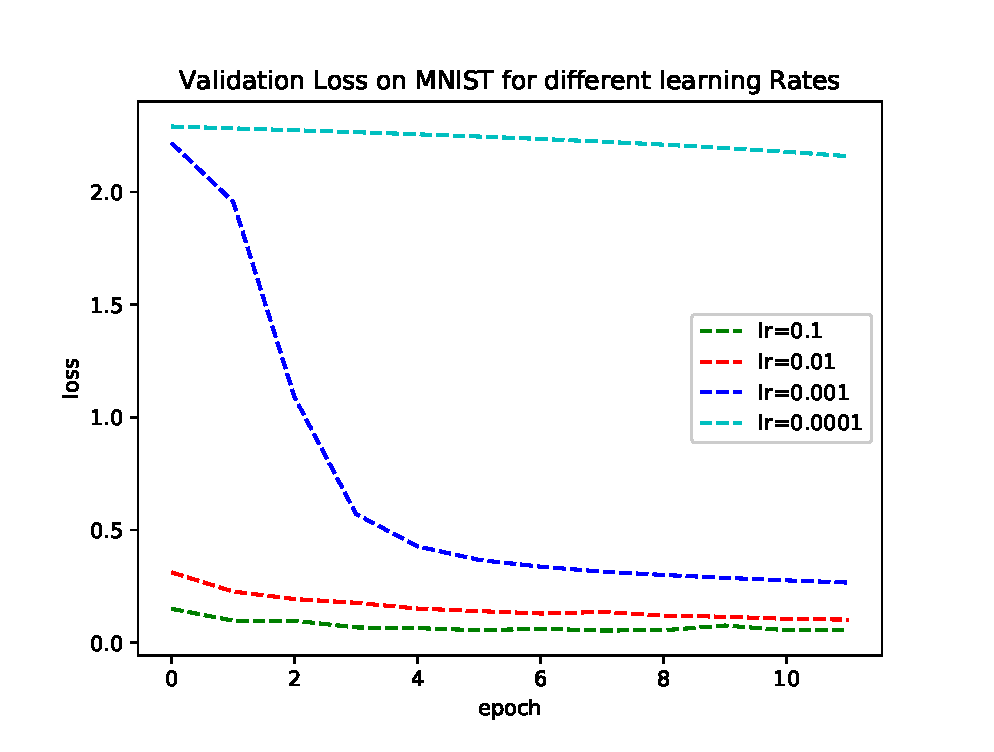
\includegraphics[scale=1]{Ex2.eps}

From that figure we can observe that the bigger learning rates lead to better results for 12 epochs. The two lower values (0.0001) also help with decreasing the loss and the error but lead to too small changes in the parameters such that the model is far from convergence after 12 epochs.
With the two higher values (0.01 and 0.1) the model has mostly converged to a local minimum after 12 epochs and thus is finished with the training. With higher learning rates the performance again could get worse if the steps are too big and we jump out of a locally optimal region. However we can not observe this behavior in this experiment. Our Random search from exercise 4 suggests that the optimal learning rate (with SGD and no annealing schedule) lies slightly below 0.1 for this scenario.
\subsection*{Exercise 3, Filter Sizes}
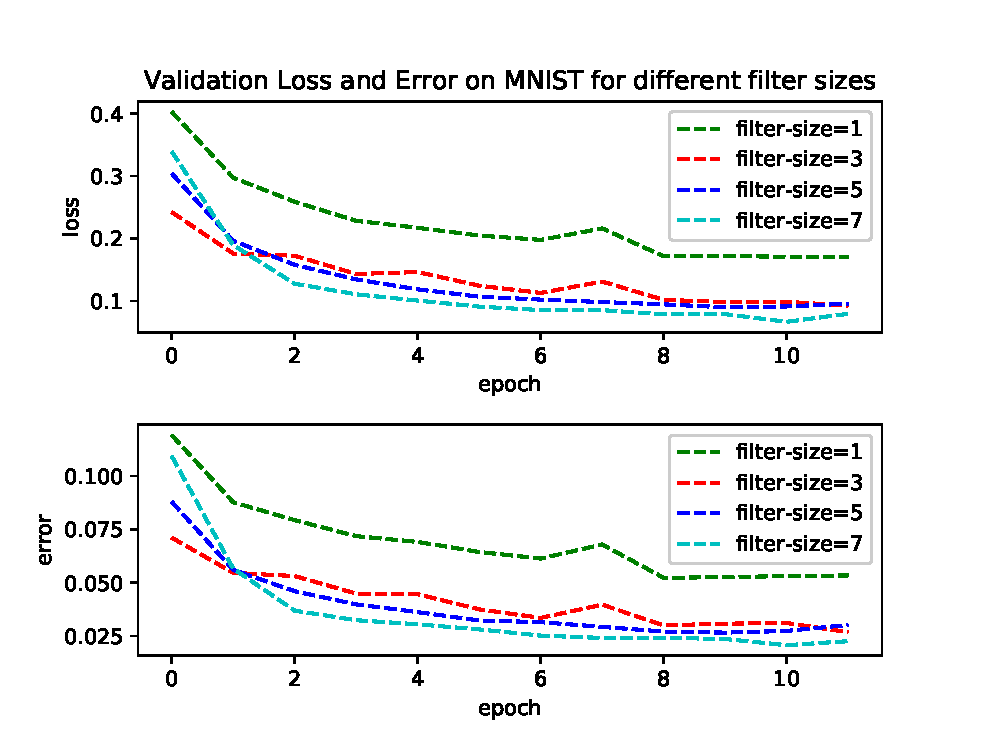
\includegraphics[scale=1]{Ex3.eps}
This picture was created with a batch size of 128 and a learning rate of 0.03. It suggests that bigger filters perform better on the mnist dataset.
However the best performance from the random search in ex. 4 was achieved by a 3x3 filter.
I would assume that smaller filters can perform better if the input resolution is lower, s.t the dependency or connection between neighboring pixels is of a short range. But this is just an assumption.

\subsection*{Exercise 4, Random Search}
The best configuration that was found during my experiments with the given settings was:
\begin{itemize}
	\item learning rate: $0.08847$
	\item batch size: 46
	\item filter size: 3x3
	\item number of filters per layer: 63
\end{itemize}
After training this setup for the full 12 epochs it achieved an error rate on the test set of \textbf{0.98\%} which is much better than what I could achieve with the feed forward networks from two weeks ago. The following plot shows the
validation error of the currently found best configuration of random search (budget of 6 epochs)\\
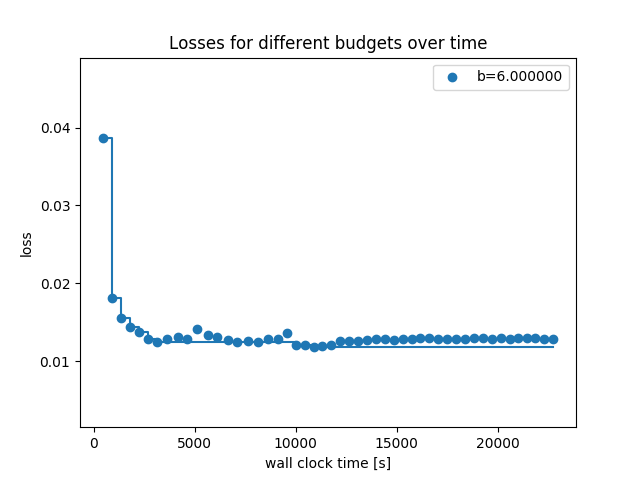
\includegraphics[scale=0.7]{random_result.png}

And the following graph shows the performance on the validation set of the best model during 12 epochs of training. \\
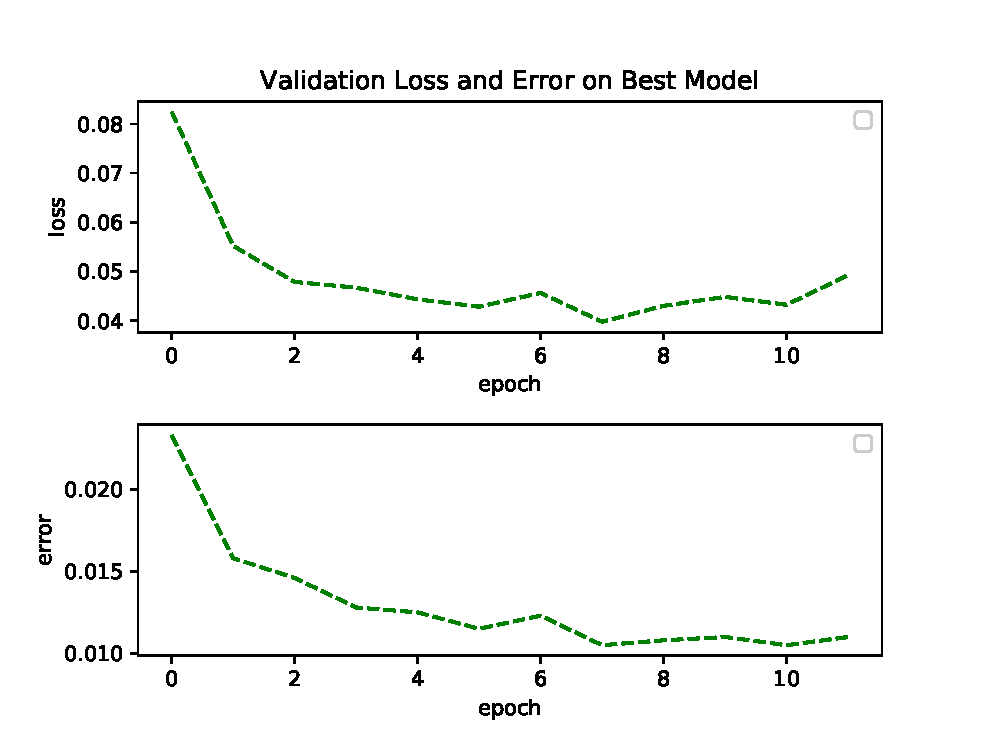
\includegraphics[scale=1]{randomPerformance.eps}
\end{document}


